\documentclass[11pt]{article}
\usepackage{graphicx}
\usepackage[margin=1in]{geometry}
\usepackage[default,oldstyle,scale=0.95]{opensans}
\usepackage{setspace}
\onehalfspacing

\author{
	George G Vega Yon \and 
	Duncan Thomas \and
	Huaiyu Mi \and
	John Morrison \and
	Paul D Thomas \and
	Paul Marjoram
}

\title{Triads, Dyads, and Gene Functions: When Social Network Analysis meets Phylogenetics}

\date{}

\begin{document}
	
	\maketitle
	
Understanding what genes do is undoubtedly one of the most pressing challenges of biomedical research. Knowing gene functions is paramount for advancing treatment development, yet, conducting experiments to augment our knowledge is both time-consuming and, many times, implausible. In this context, scientists are in a race to automatically annotate gene functions at a large scale. This paper presents a novel approach that taps into phylogenetic trees and methods developed in social network analysis to build an evolutionary model of gene functions.

%\begin{figure}[htb]
%	\centering
%	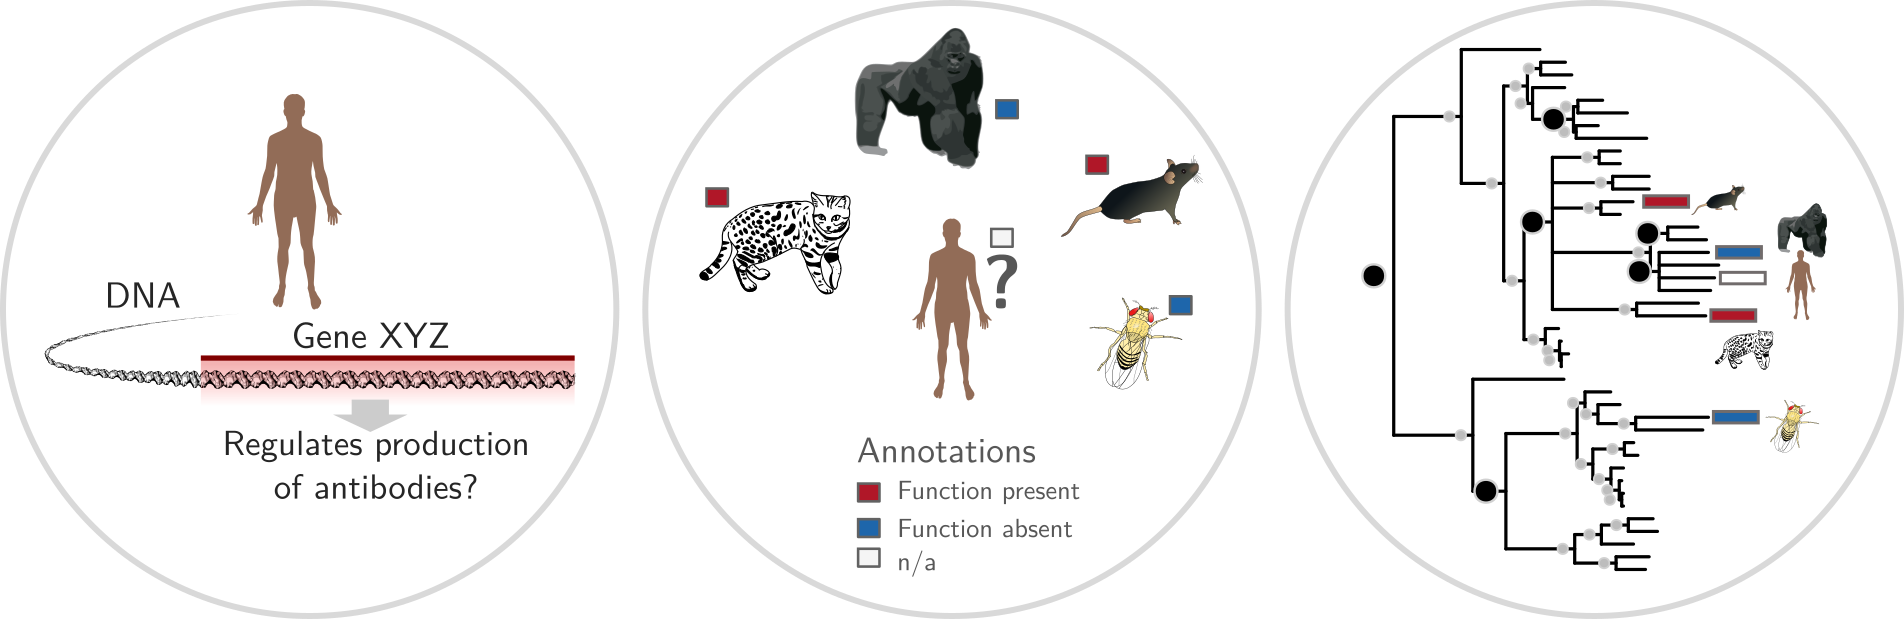
\includegraphics[width=.9\linewidth]{aphylo-data.png}
%	\caption{text}
%\end{figure}

In simple terms, phylogenetic-based prediction models allow us to borrow known gene annotations to infer others without the need to run experiments. Intuitively, if gene A's evolutionary cousin has function X, the chances are that A has the function too. Using a Markov transition model, we can characterize the evolutionary process at each step, i.e., when functions are gained or lost throughout evolution. Notwithstanding, as the number of functions we look at increases--genes can have multiple functions,--Markov transition models rapidly fall to the course of dimensionality. Instead, inspired by the ideas developed around Exponential Random Graph Models (ERGMs), we propose using sufficient statistics to simplify the problem while improving its interpretability significantly.

Without sufficient statistics, a common approach to fit this model would require estimating $2^{3k}$ parameters in a problem with $k$ gene functions. For example, if we were looking at four different functions, the procedure would involve 4096 parameters. Using sufficient statistics, we can reduce the number of parameters to as little as 15 and still incorporate complex interplay between gene functions. The only thing we ought to do is treat the transition process the same way we would do a social network. We will explain the details in our presentation.

In summary, we propose a novel approach for modeling gene function evolution using phylogenetic trees and ERGMs. This approach's main contribution is three-fold: It bypasses the curse of dimensionality experienced in canonical approaches, it provides a way to conduct hypothesis testing of different theories of evolution, and most importantly, it has the prospect of enhancing our prediction capacity using an interpretable model.


\end{document}